\chapter*{Experiment 2 - Button}
\addcontentsline{toc}{chapter}{Experiment 2 - Button}
We wire up the experiment as shown in the diagram fig:~\ref{fig:exp2_button}. And upload the sketch code in the next section on page:~\pageref{sketch:exp2}.

%
\begin{figure}[ht]
	\centering
	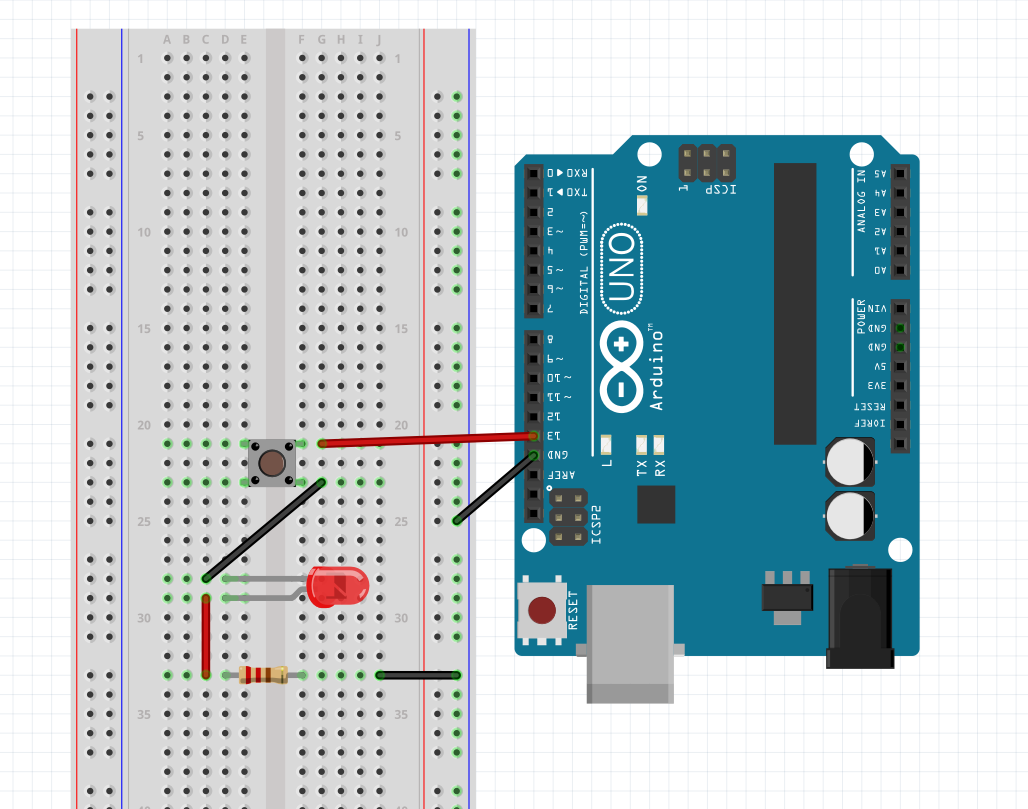
\includegraphics[width=12cm]{images/08}
	\caption{Button activated LED \citep{fritzing-15}}
	\label{fig:exp2_button}
\end{figure}
%

The LED will light up when the button is pressed.

\newpage
\section*{Sketch Code}
\label{sketch:exp2}
\begin{lstlisting}
/*
Button activated LED

This example code is in the public domain.
*/

 
// Pin 13 has an LED connected on most Arduino boards.
// give it a name:
int led = 13;

// the setup routine runs once when you press reset:
void setup() {                
  // initialize the digital pin as an output.
  pinMode(led, OUTPUT);     
}

// the loop routine runs over and over again forever:
void loop() {
  digitalWrite(led, HIGH);   // turn the LED on (HIGH is the voltage level)
}

\end{lstlisting}